\section{Fermion Parity from String Operators}\label{sec:fermion_parity_from_string_operators}

\valert{
The physical meaning of the total fermion parity in the spin representation is important, not only because the subtlety about the definition of equivalence classes arises from it, but also because of its importance when calculating the reduced density matrix.
}

String operators of edge configurations in the same class have the same magnitude of expectation values,
\[
\abs{\anglelr{\Sigma_{\mathfrak{D}}}} = \abs{\anglelr{\Sigma_{\mathfrak{D}'}}} \quad\text{if $\mathfrak{D}\sim\mathfrak{D}'$}
\]
hence contribute the same weight to the density matrix. Nevertheless, it is still possible for two configurations from different classes to have the same weight contribution to the density matrix. There are a type of plaquette configurations, $\mathfrak{P}$ and $\mathfrak{S}$, that transform an edge configuration $\mathfrak{D}$ to $\mathfrak{D}\ominus\mathfrak{D}_Z$ because of the following relation
\begin{equation}\label{equ.P-S-dimer}
    \prod_{p\in\mathfrak{P}}W_p = \prod_{p\in\mathfrak{S}}W_p = \prod_{\anglelr{ij}\in \mathfrak{D}_Z}\sigma_i^z\sigma_{j}^z = \Sigma_{\mathfrak{D}_Z}.
\end{equation}
The plaquette configurations $\mathfrak{P}$ and $\mathfrak{S}$ as well as the edge configuration $\mathfrak{D}_Z$ are illustrated in the left panel of \autoref{fig.S-P-dimer-gas}. The edge configuration $\mathfrak{D}_Z$ is composed of the $z$-directional dimers all over the system. The plaquette configuration $\mathfrak{P}$ contains all the plaquettes at the even horizontal layers, while $\mathfrak{S}$ is the complement of $\mathfrak{P}$. The endpoint configuration $\mrm{EP}(\mathfrak{D}_Z)$ is simply the set of all the lattice sites in the system. On the other hand, the operators $\prod_{p\in\mathfrak{P}}W_p$ and $\prod_{p\in \mathfrak{S}}W_p$ is also equal to the string operator of the zigzag edge configuration $\mathfrak{D}_{zz}$, a set of all the $x$- and $y$-edges, as illustrated in the right panel of \autoref{fig.S-P-dimer-gas}
\begin{equation}\label{equ.M-MZ-complement}
\prod_{p\in\mathfrak{P}}W_p = \prod_{p\in\mathfrak{S}}W_p  = \Sigma_{\mathfrak{D}_{zz}}
\end{equation}
because $\de\mathfrak{P} = \de\mathfrak{S} = \mathfrak{D}_{zz}$.  Unlike $\mathfrak{D}_Z$, this edge configuration has no endpoints, $\mrm{EP}(\mathfrak{D}_{zz})=\varnothing$, and is equivalent to vacuum. So, we need to keep in mind that every two configurations, $\mathfrak{D}\ominus\mathfrak{D}_Z$ and $\mathfrak{D}\ominus\mathfrak{D}_{zz}$, give an identical string operator, although they are not equivalent.

We would also like to show that the physical meaning of the operator $\Sigma_{\mathfrak{D}_Z}$ is the total fermion parity of the $c$-Majorana fermions. Because the expectation values of fluxes are fixed to be $\anglelr{W_p}=+1$ in the ground state, we directly know that the expectation value of $\Sigma_{\mathfrak{D}_Z}$ is equal to $+1$ directly from equation \eqref{equ.P-S-dimer} 
\begin{equation}\label{equ.fermion-parity-dimer-rep}
    \anglelr{\Sigma_{\mathfrak{D}_Z}}=1
\end{equation}
It is also worth mentioning that the combination of the plaquette operator over $\mathfrak{P}$ and the string operators containing $z$-dimers all over the lattice is equal to multiplying all edges in the entire lattice $\Lambda$ together
\begin{equation}\label{equ.fermion-parity-spin-rep}
    \lr{\prod_{p\in\mathfrak{P}}W_p} \Sigma_{\mathfrak{D}_Z} = \prod_{\anglelr{ij}\in\Lambda}\dimer{i}{j} = \mathds{1}
\end{equation}
This is nothing but the identity operator of the entire system because of the geometry of the honeycomb lattice. We can understand equations \eqref{equ.fermion-parity-dimer-rep} and \eqref{equ.fermion-parity-spin-rep} in the sense of fermion parity. In our convention, the gauge is fixed as $u_{ij}=1\forall\anglelr{ij}$, therefore, the string operator corresponding to the edge configuration that contains all of the edges in the lattice, as appeared in the last equation, transforms into the fermion parity operator $\hat{\bog{\pi}}$ up to a phase~\footnote{Two distinct Majorana fermions, say $c_1$ and $c_2$, can combine to form a normal fermion degree of freedom $f$ in a way that $f=\frac{1}{2}\lr{c_1+ic_2}$ and $f^\dagger=\frac{1}{2}\lr{c_1-ic_2}$. In this way, the fermion parity operator represented using the Majorana fermions becomes $\hat{\bog{\pi}}\equiv(-1)^{f^\dagger f}=ic_1c_2$. In a more general sense, the fermion parity operator is equal to the multiplication of all the Majorana fermions $\prod_i c_i$ up to a phase.}
\begin{equation}\label{equ.total-fermion-parity-entire-system}
    \prod_{\anglelr{ij}\in\Lambda}\dimer{i}{j}\to \prod_{\anglelr{ij}\in \Lambda}ic_ic_j
\propto \prod_{i\in\Lambda}c_i\propto \hat{\bog{\pi}}
\end{equation}
This is also due to the geometric feature of the honeycomb lattice, in which three connected edges share a lattice site. Similarly, the operator $\Sigma_{\mathfrak{D}_Z}$ in the Majorana representation is also equal to the fermion parity operator
\begin{equation}\label{equ.total-fermion-parity-Sigma-Z}
    \Sigma_{\mathfrak{D}_Z} \to \prod_{\anglelr{ij}\in\mathfrak{D}_Z}ic_ic_j\propto \prod_{i\in\Lambda}c_i\propto\hat{\bog{\pi}},
\end{equation}
because, as we will emphasize later, Majorana fermions emerge at the endpoints of each $z$-directional dimer, thus $\mrm{EP}(\mathfrak{D}_Z)$ is exactly the whole lattice system $\Lambda$. From the Majorana fermion point of view, the fermionic representation of the Kitaev Hamiltonian \eqref{equ.MF-Hamiltonian} is quadratic. As a consequence, the total fermion parity of the whole system should be conserved and must be $+1$ on a torus~\cite{Fu-Knolle-Perkins-2018}. This fermion parity degree of freedom is emergent only in the Majorana representation, and should be fixed by the intrinsic property of the spin operators in the physical spin representation. This is why the expectation value of the operator $\Sigma_{\mathfrak{D}_Z}$ is $+1$. 

\begin{figure}
    \centering
    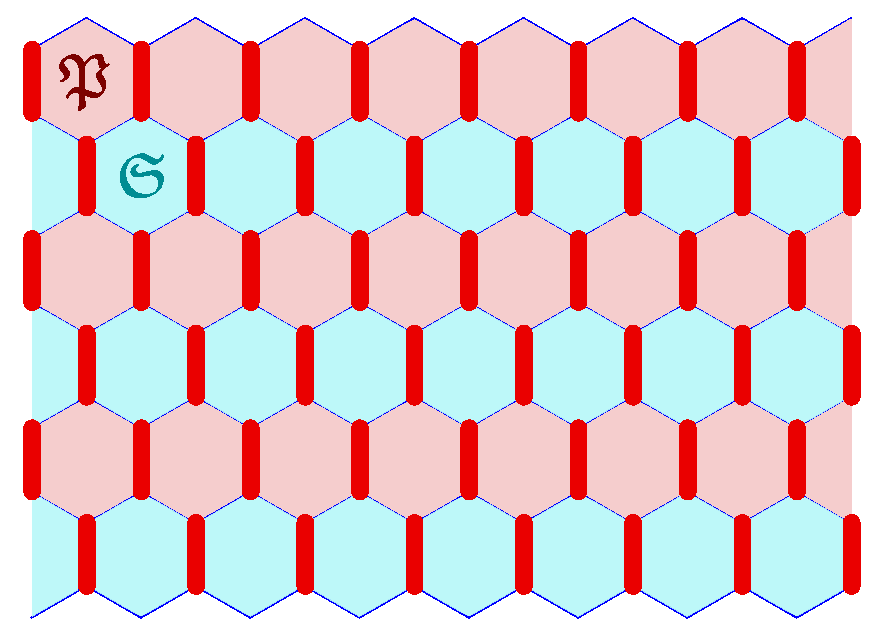
\includegraphics[width=0.48\linewidth]{figures/S-P-dimer-gas.pdf}
    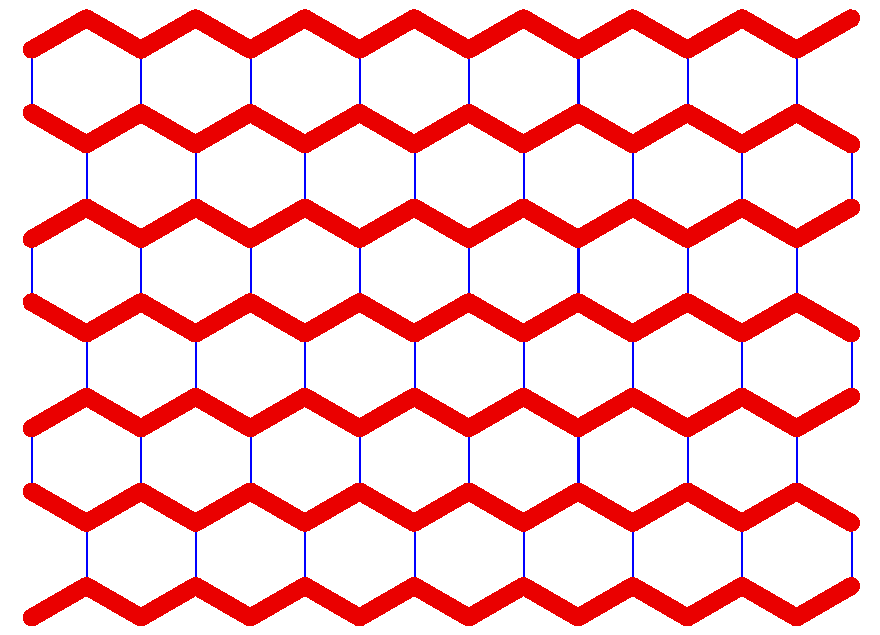
\includegraphics[width=0.48\linewidth]{figures/snake-and-dimer-gas.pdf}
    \caption{The left panel illustrates the plaqeutte configurations $\mathfrak{P}$ and $\mathfrak{S}$ as well as the edge configuration $\mathfrak{D}_Z$. The set of plaquettes in pink is denoted by $\mathfrak{P}$, while the set containing those in pink-blue is denoted by $\mathfrak{S}$. The edge configuration $\mathfrak{D}_Z$ consists of all of the red $z$-directional edges in the system, as shown in the above figure. The right panel illustrates the zigzag configuration $\mathfrak{D}_{zz}$ consisting of edges at all the horizontal loops. Such an edge configuration is also the boundary of both $\mathfrak{P}$ and $\mathfrak{S}$, for which we can write $\mathfrak{D}_{zz} = \de\mathfrak{P} = \de\mathfrak{S}$. Note that $\Sigma_{\mathfrak{D}_Z}=\Sigma_{\mathfrak{D}_{zz}}$ although $\mrm{EP}(\mathfrak{D}_Z)\neq \mrm{EP}(\mathfrak{D}_{zz})=\varnothing$} 
    \label{fig.S-P-dimer-gas}
\end{figure}